% Panel (b): radiation-induced segregation.  Generated by make_panel_b.py
% Profiles: mirrored about the GB, convolved with a 1 nm FWHM Gaussian,
% right half shown.  Schematic - axes deliberately omitted.
\documentclass[12pt,border=2pt,tikz]{standalone}

\usepackage{amsmath}
\newcommand{\Vac}{\mathrm{V}}
\newcommand{\Int}{\mathrm{I}}
\newcommand{\lat}{\mathrm{lat}}
\usetikzlibrary{arrows.meta}

\definecolor{cMetal}{RGB}{214,214,211}
\definecolor{cEdge}{RGB}{40,40,44}
\definecolor{cGB}{RGB}{96,42,140}
\definecolor{cCr}{RGB}{17,119,51}
\definecolor{cNi}{RGB}{0,90,181}
\definecolor{cSi}{RGB}{214,96,20}

\begin{document}
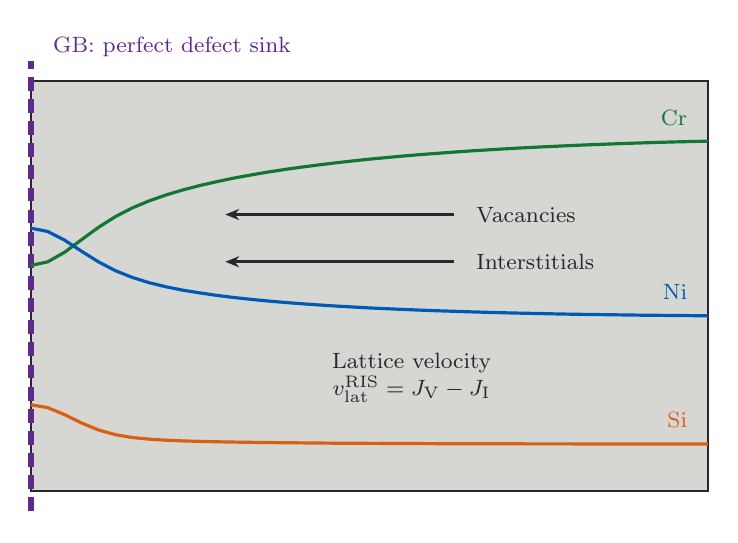
\begin{tikzpicture}[
  x=1cm,y=1cm, font=\footnotesize, color=cEdge,
  eg/.style   ={draw=cEdge, line width=0.8pt},
  prof/.style ={line width=1.15pt, line join=round},
  defect/.style={-{Stealth[length=5pt,width=4pt]}, line width=1.0pt, draw=cEdge},
]

\def\W{8.60}\def\H{5.20}

% ----- metal domain ----------------------------------------------------
\fill[cMetal,eg] (0,0) rectangle (\W,\H);

% ----- the GB: a plane that acts as a perfect defect sink ---------------
\draw[cGB,line width=2.2pt,dash pattern=on 5pt off 3pt]
      (0,-0.26) -- (0,\H+0.26);
\node[anchor=west,cGB] at (0.16,\H+0.44) {GB: perfect defect sink};

% ----- point-defect fluxes towards the boundary ------------------------
\draw[defect] (5.375,3.509) -- (2.472,3.509);
\node[anchor=west] at (5.535,3.509) {Vacancies};
\draw[defect] (5.375,2.909) -- (2.472,2.909);
\node[anchor=west] at (5.535,2.909) {Interstitials};

% ----- segregation profiles --------------------------------------------
\draw[prof,cCr] plot coordinates {(0.000,2.862) (0.215,2.908) (0.430,3.030) (0.645,3.189) (0.860,3.346) (1.075,3.482) (1.290,3.593) (1.505,3.683) (1.720,3.758) (1.935,3.822) (2.150,3.878) (2.365,3.927) (2.580,3.972) (2.795,4.011) (3.010,4.048) (3.225,4.081) (3.440,4.111) (3.655,4.139) (3.870,4.165) (4.085,4.189) (4.300,4.212) (4.515,4.232) (4.730,4.252) (4.945,4.270) (5.160,4.286) (5.375,4.302) (5.590,4.317) (5.805,4.330) (6.020,4.343) (6.235,4.355) (6.450,4.366) (6.665,4.376) (6.880,4.386) (7.095,4.395) (7.310,4.403) (7.525,4.411) (7.740,4.418) (7.955,4.425) (8.170,4.431) (8.385,4.436) (8.600,4.441)};
\draw[prof,cNi] plot coordinates {(0.000,3.336) (0.215,3.294) (0.430,3.184) (0.645,3.043) (0.860,2.908) (1.075,2.796) (1.290,2.710) (1.505,2.643) (1.720,2.591) (1.935,2.548) (2.150,2.513) (2.365,2.482) (2.580,2.455) (2.795,2.432) (3.010,2.411) (3.225,2.393) (3.440,2.376) (3.655,2.361) (3.870,2.347) (4.085,2.335) (4.300,2.323) (4.515,2.313) (4.730,2.304) (4.945,2.295) (5.160,2.287) (5.375,2.280) (5.590,2.273) (5.805,2.267) (6.020,2.261) (6.235,2.256) (6.450,2.252) (6.665,2.247) (6.880,2.243) (7.095,2.240) (7.310,2.237) (7.525,2.234) (7.740,2.231) (7.955,2.229) (8.170,2.227) (8.385,2.225) (8.600,2.223)};
\draw[prof,cSi] plot coordinates {(0.000,1.093) (0.215,1.057) (0.430,0.968) (0.645,0.862) (0.860,0.773) (1.075,0.713) (1.290,0.677) (1.505,0.656) (1.720,0.643) (1.935,0.634) (2.150,0.628) (2.365,0.623) (2.580,0.619) (2.795,0.616) (3.010,0.613) (3.225,0.611) (3.440,0.609) (3.655,0.607) (3.870,0.605) (4.085,0.604) (4.300,0.603) (4.515,0.602) (4.730,0.601) (4.945,0.600) (5.160,0.599) (5.375,0.599) (5.590,0.598) (5.805,0.598) (6.020,0.597) (6.235,0.597) (6.450,0.596) (6.665,0.596) (6.880,0.596) (7.095,0.595) (7.310,0.595) (7.525,0.595) (7.740,0.595) (7.955,0.595) (8.170,0.595) (8.385,0.595) (8.600,0.595)};

\node[align=center] at (4.837,1.430)
      {Lattice velocity\\ $v_{\lat}^{\mathrm{RIS}}=J_{\Vac}-J_{\Int}$};

\node[anchor=east,cCr] at (\W-0.14,4.741) {Cr};
\node[anchor=east,cNi] at (\W-0.14,2.523) {Ni};
\node[anchor=east,cSi] at (\W-0.14,0.895) {Si};

\end{tikzpicture}
\end{document}
